%! Author = Len Washington III
%! Date = 11/11/24

% Preamble
\documentclass[
	date={November 11{,} 2024},
	month={11},
	day={11}
]{math486notes}
\usetikzlibrary{arrows.meta}

% Document
\begin{document}

\tableofcontents

Parameter fitting or Calibration.

Crucial step in modeling (machine learning).
Theory $\rightarrow$ practice.

Compartment models (linear) \_\_\_ to functions that are sums of exponentials

\begin{equation}
	\begin{aligned}
		x(t) &= c_{1}e^{-\lambda_{1}t} + c_{2}e^{-\lambda_{2}t}\\
		&= f(t, c_{1}, c_{2}, \lambda_{1}, \lambda_{2})
	\end{aligned}
	\label{eq:22-1}
\end{equation}
Given training data $\{t_{i}, x_{i}\}_{i=1}^{N}$

If there was only 1 exponential
\begin{equation}
	x = c_{1}e^{-\lambda_{1}t}
	\label{eq:22-2}
\end{equation}

Linear: $\ln x = -\lambda_{1}t + \ln c_{1}$

\begin{enumerate}
	\item Closest solution: $A^{T}A\vec{y} = A^{T}\vec{b}$
	\item Minimize the sum of squares of the errors (SSE)
	\[ SSE = \sum_{i=1}^{N} \left[ -\lambda t_{i} + b - \ln x_{i} \right]^{2} \]
\end{enumerate}

Could try
\begin{equation*}
\begin{aligned}
	\min SSE &= \min \sum_{i=1}^{N} \left( x(t_{i}) - x_{i} \right)^{2}\\
	&= F(c_{1}, \lambda_{1}, c_{2}, \lambda_{2})
\end{aligned}
\end{equation*}

Alternate method:

\section{Exponential peeling}\label{sec:exponential-peeling}
\begin{equation}
	x(t) = c_{1}e^{-\lambda_{1} t} + c_{2}e^{-\lambda_{2} t}\ \ \ \ \ \lambda_{x} > 0\\
	\label{eq:22-4}
\end{equation}

Assume $|\lambda_{2}| > |\lambda_{1}|$.

If $t \gg 1$: $x(t) \approx c_{1}e^{-\lambda_{1} t}$ i.e. $e^{-\lambda_{2}t} \dots$

$x(t)$ is asymptotic to $c_{1}e^{\lambda_{1}t}$

\begin{figure}[H]
	\centering
	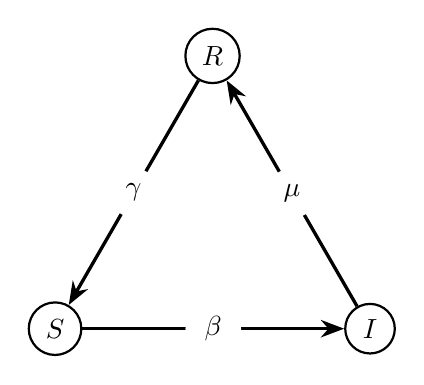
\begin{tikzpicture}[scale=2]
		\begin{scope}[every node/.style={circle,thick,draw}]
			\node (S) at (0,0) {$S$};
			\node (I) at (2,0) {$I$};
			\node (R) at (1,1.732) {$R$};
		\end{scope}
		\begin{scope}[>={Stealth[black]},
			every node/.style={fill=white,circle},
			every edge/.style={draw=black,very thick}]
			\path [->] (S) edge node {$\beta$} (I);
			\path [->] (I) edge node {$\mu$} (R);
			\path [->] (R) edge node {$\gamma$} (S);
		\end{scope}
	\end{tikzpicture}
	\caption{SIRS Model}
	\label{fig:sirs-model-2}
\end{figure}

Let $S$, $I$, $R$ be fractions (already sealed) (i.e. $S+I+R=1$)

\begin{equation*}
	\begin{aligned}
		\frac{dS}{dt} &= -\beta SI + \gamma R\\
		\frac{dI}{dt} &= \beta SI - \mu I\\
		\frac{dR}{dt} &= \mu I - \gamma R
	\end{aligned}
\end{equation*}

\begin{equation*}
	\begin{aligned}
		\frac{dS}{d\tau} &= -R_{0}SI + c(1 - I - S)\\
		&= F(S, 1)\\
		\frac{dI}{d\tau} &= R_{0}SI - I\\
		&= G(S, 1)\\
	\end{aligned}
\end{equation*}
where $\tau = \mu t$, $R_{0} = \frac{\beta}{\mu}$, $c = \frac{\gamma}{\mu}$% I = 0 or S = 1/R_{0},

\begin{equation*}
	\begin{aligned}
		\frac{dS}{dt} &= dN -\beta \frac{I}{N} S - dS\\
		\frac{dI}{dt} &= \beta \frac{I}{N} S - \mu I - dI\\
		\frac{dR}{dt} &= \mu I - \gamma R - dR
	\end{aligned}
\end{equation*}

\section{Next COVID Model -- SEIR}\label{sec:next-covid-model----seir}
$E = $ Exposed -- latent infection period

\begin{figure}[H]
	\centering
	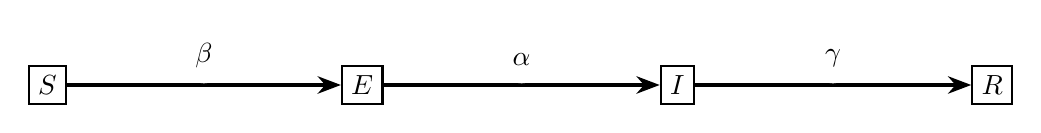
\begin{tikzpicture}[scale=2]
		\begin{scope}[every node/.style={thick,draw}]
			\node (S) at (0,0) {$S$};
			\node (E) at (2,0) {$E$};
			\node (I) at (4,0) {$I$};
			\node (R) at (6,0) {$R$};
		\end{scope}
		\begin{scope}[>={Stealth[black]},
			every node/.style={fill=white,circle},
			every edge/.style={draw=black,very thick}]
			\path [->] (S) edge node[above] {$\beta$} (E);
			\path [->] (E) edge node[above] {$\alpha$} (I);
			\path [->] (I) edge node[above] {$\gamma$} (R);
		\end{scope}
	\end{tikzpicture}
	\caption{SEIR Model}
	\label{fig:seir-model}
\end{figure}

\begin{equation*}
\begin{aligned}
	\frac{dS}{dt} &= -\beta IS,	\sep S(0) = S_{0}\\
	\frac{dE}{dt} &= \beta IS - \alpha E, \sep E(0) = E_{0}\\
	\frac{dI}{dt} &= \alpha E - \gamma I, \sep I(0) = I_{0}\\
	\frac{dR}{dt} &= \gamma I
\end{aligned}
\end{equation*}

Conservation Law: $S + E + I + R = 1$

\end{document}